% Compilazione: pdflatex -jobname=fisica_tex fisica.tex
\documentclass[a4paper,11pt]{article}
\usepackage[T1]{fontenc}
\usepackage[utf8]{inputenc}
\usepackage[margin=20mm]{geometry}
\usepackage{amsmath,amssymb,multicol,tikz,circuitikz}
\usetikzlibrary{arrows.meta,patterns}
\setlength{\parindent}{0pt}
\setlength{\parskip}{5pt}
\newcommand{\orig}[1]{\clearpage}
\newcommand{\nota}[1]{\par\small\textit{Nota di trascrizione: #1}\par\normalsize}
\newcommand{\vv}[1]{\vec{#1}}
\newcommand{\dd}{\mathrm{d}}
\begin{document}
% Pagina originale 1
\section*{Legenda}
\begin{multicols}{2}
\begin{enumerate}
\item Cinematica\begin{itemize}\item Moto rettilineo uniforme\item Moto rettilineo uniformemente accelerato\item Gittata\item Moto circolare uniforme\item Moto armonico\item Moto relativo\end{itemize}
\item Dinamica\begin{itemize}\item Principio di conservazione della quantità di moto\item Forza peso\item Reazione vincolare\item Attrito\item Forza elastica\item Tensione\item Pendolo semplice\end{itemize}
\item Energia\begin{itemize}\item Cinetica\item Lavoro\item Th. delle Forze vive\item Th. delle Forze conservative\item Potenziale\item Meccanica\item Forze conservative\item Potenza\item Quantità di moto\item Leggi di conservazione\end{itemize}
\item Sistema di particelle\begin{itemize}\item Momento angolare\item Momento torcente\item Th. di König\end{itemize}
\item Urti\begin{itemize}\item Elastico\item Anelastico\item Completamente anelastico\end{itemize}
\item Corpo rigido\begin{itemize}\item Momento di inerzia\item Th. di Huygens-Steiner\item Equilibrio statico\end{itemize}
\item Gravitazione\begin{itemize}\item Formula gravitazionale\item Leggi di Keplero\end{itemize}
\item Pendolo fisico
\item Elettrostatica\begin{itemize}\item Legge di Coulomb\item Campo elettrostatico\item Legge di Gauss\item Energia Potenziale elettrica\item Potenziale elettrico\end{itemize}
\item Circuiti\begin{itemize}\item Capacità\item Resistenza\item Corrente\item Potenza\end{itemize}
\item Magnetismo\begin{itemize}\item Legge di Biot-Savart\item Effetto Hall\item Legge di Ampere\item Legge di Faraday\item Forza di Lorentz\end{itemize}
\item Induttanza
\item Equazioni di Maxwell
\item Carica e scarica dei Condensatori\begin{itemize}\item Carica\item Scarica\end{itemize}
\end{enumerate}\end{multicols}
% Pagina originale 2
\orig{2}
\section*{Cinematica}
\begin{align*}
x(t)&=x_0+v_0t+\tfrac12at^2 &&\text{moto uniformemente acc.}\\
x(t)&=x_0+v_0t &&\text{moto rettilineo uniforme}\\
v(t)&=\text{cost.}\quad\text{(uniforme)},&v(t)&=v_0+at\quad\text{(unif. acc.)}\\
v&=\frac{\dd x}{\dd t},&a&=\frac{\dd v}{\dd t}=\frac{\dd^2x}{\dd t^2}.
\end{align*}
\subsection*{Gittata}
\[G=\frac{v_0^2}{g}\sin 2\theta.\]
\begin{center}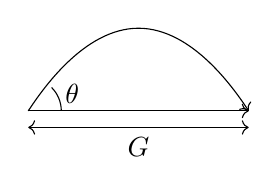
\begin{tikzpicture}[scale=.7]\draw[->] (0,0)--(4,0);\draw[->] (0,0) parabola bend (2,1.5) (4,0);\draw[<->] (0,-.3)--node[below]{$G$}(4,-.3);\draw (0.6,0) arc (0:45:.6);\node at (.8,.3){$\theta$};\end{tikzpicture}\end{center}
\subsection*{Moto circolare uniforme}
Velocità e acc. costanti in modulo.
\[\omega=\frac{2\pi}{T}=2\pi\nu\quad[\mathrm{rad/s}],\qquad \omega=\frac vR.\]
\[a_c=\frac{v^2}{R}=\omega^2R,\qquad a_T=0,\qquad \alpha=\frac{a_T}{R}.\]
\begin{center}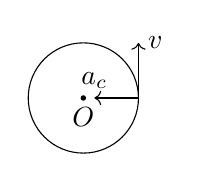
\begin{tikzpicture}[scale=.7]\draw (0,0) circle(1);\fill (0,0) circle(.05) node[below]{$O$};\draw[->](1,0)--(1,1) node[right]{$v$};\draw[->](1,0)--(.2,0) node[above]{$a_c$};\end{tikzpicture}\end{center}
\[\theta(t)=\theta_0+\omega t+\tfrac12\alpha t^2\quad\text{acc. cost. (angolare)},\qquad
\theta(t)=\theta_0+\omega t\quad\text{vel. cost.}\]
\subsection*{Moto armonico (per le molle)}
\[T=\frac1\nu=\frac{2\pi}{\omega}=\frac{2\pi r}{v},\qquad \nu=\frac1T=\frac{\omega}{2\pi}\quad[\mathrm{Hz}].\]
\[x(t)=\underbrace{A}_{\text{ampiezza massima}}\sin(\underbrace{\omega}_{\text{pulsazione angolare}}t+\underbrace{\varphi}_{\text{fase iniziale}}).\]
\[v(t)=\frac{\dd x}{\dd t}=\omega A\cos(\omega t+\varphi),\qquad
 a(t)=\frac{\dd v}{\dd t}=-\omega^2A\sin(\omega t+\varphi)=-\omega^2x(t).\]
\begin{center}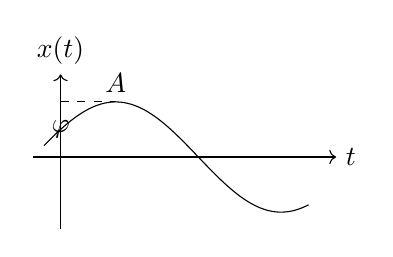
\begin{tikzpicture}[scale=.7]\draw[->](-.5,0)--(5,0)node[right]{$t$};\draw[->](0,-1.3)--(0,1.5)node[above]{$x(t)$};\draw[domain=-.3:4.5,samples=80]plot(\x,{sin((\x+.5)*60)});\draw[dashed](0,1)--(1,1)node[above]{$A$};\node at (0,.5){$\varphi$};\end{tikzpicture}\end{center}

% Pagina originale 3
\orig{3}
\subsection*{Moto relativo}
\[\underbrace{a_A}_{\text{assoluta}}=\underbrace{a'}_{\text{relativa}}+\underbrace{a_T}_{\text{di trascinamento}}.\]
\section*{Dinamica}
\begin{enumerate}
\item $p=mv$ (q.tà di moto). Principio di conservazione della q.tà di moto $p$.
\item $F=\dd p/\dd t$ (se $\dd m/\dd t=m$ ($m$ cost.) $\Rightarrow F=ma$). Forze applicate producono accelerazione.
\item $F_{AB}=-F_{BA}$ (azione e reazione).
\end{enumerate}
\nota{La condizione manoscritta al punto 2 è riportata letteralmente: sembra scrivere $\dd m/\dd t=m$, pur annotando ``$m$ cost.''.}
\textbf{Forza peso:}\quad $P=-mg$.

\textbf{Reazione vincolare:}\quad $\vv N+\vv f_{\mathrm{appl},y}=\vv0$.
\begin{center}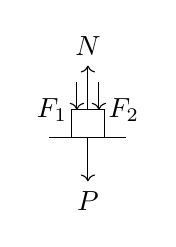
\begin{tikzpicture}[scale=.7]\draw(-.7,0)--(.7,0);\draw(-.3,0)rectangle(.3,.5);\draw[->](0,.5)--(0,1.3)node[above]{$N$};\draw[->](0,0)--(0,-.8)node[below]{$P$};\draw[->](-.2,1)--(-.2,.5)node[left]{$F_1$};\draw[->](.2,1)--(.2,.5)node[right]{$F_2$};\end{tikzpicture}\end{center}
\textbf{Attrito:}\quad $F_{\mathrm{att}}=\mu N$;
statico: $F_s\leq\mu_sN$; dinamico: $F_d=\mu_dN$ ($\mu_d<\mu_s$).

\textbf{Forza elastica:}\quad $\vv F_{\mathrm{el}}=-k\vv x$ (legge di Hooke), con $x-l_0$.
\[x(t)=|A|\sin(\omega t+\varphi)\quad\text{(moto armonico)},\qquad \omega=\sqrt{\frac km}.\]
\textbf{Tensione:}\quad $\vv T=-\vv f_{\mathrm{appl}}$.
\begin{center}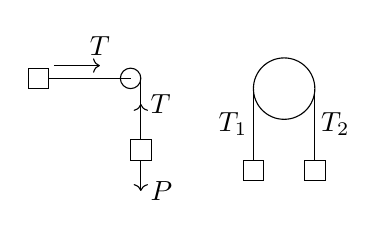
\begin{tikzpicture}[scale=.65]\draw(0,0)rectangle(.4,.4);\draw(.4,.2)--(2,.2);\draw(2,.2)circle(.2);\draw(2.2,.2)--(2.2,-1);\draw(2,-1)rectangle(2.4,-1.4);\draw[->](.5,.45)--(1.4,.45)node[above]{$T$};\draw[->](2.2,-.8)--(2.2,-.3)node[right]{$T$};\draw[->](2.2,-1.4)--(2.2,-2)node[right]{$P$};\draw(5,0)circle(.6);\draw(4.4,0)--(4.4,-1.4);\draw(5.6,0)--(5.6,-1.4);\draw(4.2,-1.4)rectangle(4.6,-1.8);\draw(5.4,-1.4)rectangle(5.8,-1.8);\node at (4,-.7){$T_1$};\node at (6,-.7){$T_2$};\end{tikzpicture}\end{center}
$T_1=T_2$ se $a=0$ o carrucola ideale.
\subsection*{Pendolo semplice}
\begin{center}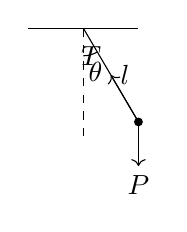
\begin{tikzpicture}[scale=.7]\draw(-1,0)--(1,0);\draw[dashed](0,0)--(0,-2);\draw(0,0)--(1,-1.7)node[midway,right]{$l$};\fill(1,-1.7)circle(.08);\draw[->](1,-1.7)--(.5,-.85)node[above left]{$T$};\draw[->](1,-1.7)--(1,-2.5)node[below]{$P$};\draw(0,-.5)arc(-90:-60:.5);\node at(.22,-.8){$\theta$};\end{tikzpicture}\end{center}
\[\begin{cases}T-mg\cos\theta=ma_R=m\omega^2l &\text{radiale},\\-mg\sin\theta=ma_T=m\dfrac{\dd^2}{\dd t^2}(l\theta).\end{cases}\]
\[T=2\pi\sqrt{\frac lg},\qquad \theta(t)=\theta_{\max}\cos(\Omega t+\varphi),\quad \Omega=\sqrt{\frac gl}.\]
% Pagina originale 4
\orig{4}\section*{Energia}
\textbf{Cinetica:}\quad $K=\tfrac12mv^2$.

\textbf{Lavoro:}\quad $L=\vv F\cdot\vv s\ [\mathrm J]=F\,s\cos\theta$.
\[\vv F\parallel\vv s\Rightarrow L\text{ max};\qquad \vv F\perp\vv s\Rightarrow L=0.\]
\textbf{Th. delle forze vive:}
\[L=\Delta K=K_f-K_i=\tfrac12m(v_f^2-v_i^2).\]
\textbf{Th. forze conservative:}\quad $L=-\Delta U=U_i-U_f=\text{[annotazione cancellata]}$.

\textbf{Potenziale:}\quad forza peso $U=mgh$; forza elastica $U=\tfrac12k(x-l_0)^2$.

\textbf{E. meccanica:}\quad $E_m=U+K$.

\textbf{Forze conservative:}\quad $\Delta E_m=0\Longleftrightarrow$ si applicano solo f. cons.

\textbf{Potenza:}\quad $P=\dfrac{\dd L}{\dd t}=\vv F\cdot\vv v$.
\[\Delta E_m=F_{\text{non conservative}}.\]
\nota{L'ultima uguaglianza è scritta con $F$ nella fonte, senza un fattore spostamento o un simbolo di lavoro.}
\subsection*{Q.tà di moto}
\[p=m\cdot v,\qquad \underbrace I_{\text{impulso}}=\Delta p=p_f-p_i=F\cdot\Delta t=\int_{t_i}^{t_f}F\,\dd t.\]
\subsection*{Leggi di conservazione}
\[\begin{aligned}p\text{ cost.}&\Longleftrightarrow\sum F_{\mathrm{ext}}=0,\\
L_T\text{ cost.}&\Longleftrightarrow\sum\tau=0,\\
E\text{ cost.}&\Longleftrightarrow\sum L_{\text{non cons.}}=0.\end{aligned}\]
% Pagina originale 5
\orig{5}\section*{Sistema di particelle}
\[x_{\mathrm{CM}}=\frac{\sum x_im_i}{\sum m_i}=\frac{x_1m_1+x_2m_2+\cdots+x_nm_n}{m_1+m_2+\cdots+m_n}.\]
\[v_{\mathrm{CM}}=\frac{\sum v_im_i}{\sum m_i}\Rightarrow Mv_{\mathrm{CM}}=\sum_i v_im_i.\]
Sistema isolato $\Rightarrow p$ costante.
\[a_{\mathrm{CM}}=\frac{\sum a_im_i}{\sum m_i}\Rightarrow Ma_{\mathrm{CM}}=\sum a_im_i.\]
\subsection*{Momento angolare}
\[\vv L=\vv r\wedge\vv p=m\vv r\wedge\vv v,\qquad L\perp\text{ al piano del foglio}.\]
Nel moto circolare: $L=mrv=mr^2\omega$.
\subsection*{Momento torcente}
\[\vv\tau=\vv r\wedge\vv F,\qquad r\parallel F\Rightarrow\tau=0,\qquad r\perp F\Rightarrow\tau\text{ max}.\]
\begin{center}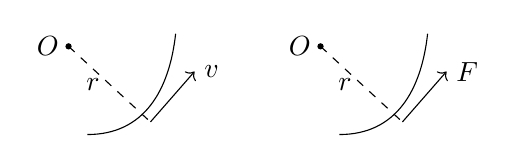
\begin{tikzpicture}[scale=.8]\fill(0,1.4)circle(.05)node[left]{$O$};\draw[dashed](0,1.4)--(1.3,.2)node[midway,left]{$r$};\draw(.3,0)..controls(1.2,0)and(1.6,.7)..(1.7,1.6);\draw[->](1.3,.2)--(2,1)node[right]{$v$};\begin{scope}[xshift=4cm]\fill(0,1.4)circle(.05)node[left]{$O$};\draw[dashed](0,1.4)--(1.3,.2)node[midway,left]{$r$};\draw(.3,0)..controls(1.2,0)and(1.6,.7)..(1.7,1.6);\draw[->](1.3,.2)--(2,1)node[right]{$F$};\end{scope}\end{tikzpicture}\end{center}
\[\Delta L=\vv r\wedge\underbrace{\vv I}_{\text{impulso}},\qquad M=\frac{\dd L}{\dd t}.\]
\[M_{\mathrm{ext}}=0\Rightarrow L\text{ cost.}\]
\textbf{Th. di König:}\quad $\vv L=\vv L^{*}+M\vv r_{\mathrm{CM}}\wedge\vv v_{\mathrm{CM}}$.
% Pagina originale 6
\orig{6}\section*{Urti}
\begin{itemize}
\item Elastico: conservazione q.tà di moto, $m_iv_i=m_fv_f$; conservazione energia cinetica, $\tfrac12m_iv_i^2=\tfrac12m_fv_f^2$.
\item Anelastico: conservazione q.tà di moto, $m_iv_i=m_fv_f$; energia rilasciata in deformazioni o esplosioni.
\item Compl. anelastico: conserv. q.tà di moto; i corpi collisi sono attaccati; $m_iv_i=(m_1+m_2)v_f$.
\end{itemize}
\[m_1v_{1i}+m_2v_{2i}=m_1v_{1f}+m_2v_{2f}.\]
\[\begin{cases}m_iv_i=m_fv_f,\\\tfrac12m_iv_i^2=\tfrac12m_fv_f^2\end{cases}\Rightarrow
\begin{cases}v_{1f}=\dfrac{m_1-m_2}{m_1+m_2}v_{1i}+\dfrac{2m_2}{m_1+m_2}v_{2i},\\[6pt]
v_{2f}=\dfrac{2m_1}{m_1+m_2}v_{1i}+\dfrac{m_2-m_1}{m_1+m_2}v_{2i}.\end{cases}\]
\section*{Corpo rigido}
\[m=\int_V\underbrace\rho_{\text{densità}}\,\dd V.\]
Se $\rho$ è costante: 1 dim. $\lambda=m/l$; 2 dim. $\sigma=m/S$; 3 dim. $\rho=m/V$.

$\rho$ costante $\Rightarrow x_{\mathrm{CM}}$ corrisponde al centro geometrico.
\subsection*{Momento di inerzia}
\[E_K=\tfrac12 I\omega^2\qquad (I\sim m,\ \omega\sim v).\]
$I$: momento d'inerzia; cambiano formule per ogni figura geometrica.
\begin{center}\begin{tabular}{ll}
Anello, asse centrale / diametro &$I_a=MR^2,\ I_v=\tfrac12MR^2$\\
Cilindro cavo &$I=\tfrac12M(R_1^2+R_2^2)$\\
Cilindro, asse longitudinale &$I_h=\tfrac12MR^2$\\
Cilindro, asse trasversale &$I_v=\tfrac14MR^2+\tfrac1{12}Ml^2$\\
Asta, asse all'estremità &$I=\tfrac13ML^2$\\
Sfera piena &$I=\tfrac25MR^2$\\
Sfera vuota &$I=\tfrac23MR^2$\\
Lastra rettangolare &$I=\tfrac1{12}M(a^2+b^2)$
\end{tabular}\end{center}
\begin{center}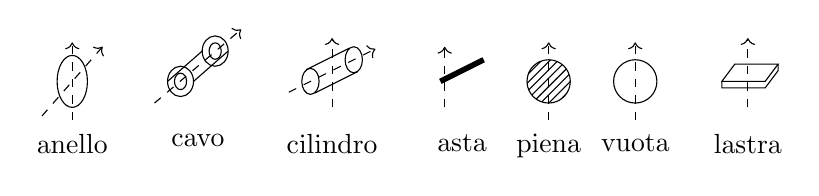
\begin{tikzpicture}[scale=.55]
\draw(0,0)ellipse(.35 and .6);\draw[dashed,->](-.7,-.8)--(.7,.8);\draw[dashed,->](0,-.9)--(0,.9);\node[below]at(0,-1){anello};
\begin{scope}[xshift=2.5cm]\draw(0,0)ellipse(.3 and .35);\draw(0,0)ellipse(.14 and .19);\draw(.8,.7)ellipse(.3 and .35);\draw(.8,.7)ellipse(.14 and .19);\draw(-.3,0)--(.5,.7);\draw(.3,0)--(1.1,.7);\draw[dashed,->](-.6,-.5)--(1.4,1.2);\node[below]at(.4,-1){cavo};\end{scope}
\begin{scope}[xshift=5.5cm]\draw(0,0)ellipse(.2 and .3);\draw(1,.5)ellipse(.2 and .3);\draw(-.1,.27)--(.9,.77);\draw(.1,-.27)--(1.1,.23);\draw[dashed,->](-.5,-.25)--(1.5,.75);\draw[dashed,->](.5,-.6)--(.5,1);\node[below]at(.5,-1){cilindro};\end{scope}
\begin{scope}[xshift=8.5cm]\draw[line width=2pt](0,0)--(1,.5);\draw[dashed,->](.1,-.6)--(.1,.8);\node[below]at(.5,-1){asta};\end{scope}
\begin{scope}[xshift=11cm]\draw[pattern=north east lines](0,0)circle(.5);\draw[dashed,->](0,-.9)--(0,.9);\node[below]at(0,-1){piena};\end{scope}
\begin{scope}[xshift=13cm]\draw(0,0)circle(.5);\draw[dashed,->](0,-.9)--(0,.9);\node[below]at(0,-1){vuota};\end{scope}
\begin{scope}[xshift=15cm]\draw(0,0)--(1,0)--(1.3,.4)--(.3,.4)--cycle;\draw(0,0)--(0,-.15)--(1,-.15)--(1.3,.25)--(1.3,.4);\draw[dashed,->](.6,-.6)--(.6,1);\node[below]at(.6,-1){lastra};\end{scope}
\end{tikzpicture}\end{center}
\textbf{Th. Huygens--Steiner:}\quad $I_P=I_{\mathrm{CM}}+Md^2$.
\nota{I disegni della fonte identificano le forme della tabella; il pedice del primo asse dell'anello è incerto (reso $a$).}
% Pagina originale 7
\orig{7}
\[\sum\tau=I\alpha\quad\text{(analoga a $\sum F=ma$)}.\]
\[\underbrace L_{\text{lavoro}}=\int\tau\,\dd\theta=\tau\Delta\theta\quad (\approx\text{ il }I=F\Delta t).\]
\[L_z=I\cdot\omega\qquad\approx mv\quad\text{q.tà di moto}.\]
\subsection*{Eq. statica}
\[\begin{cases}\sum F=0,\\\sum\tau=0.\end{cases}\]
\begin{center}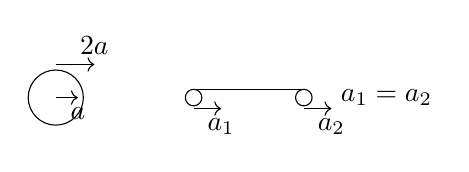
\begin{tikzpicture}[scale=.7]\draw (0,0)circle(.5);\draw[->](0,.6)--(.7,.6)node[above]{$2a$};\draw[->](0,0)--(.4,0)node[below]{$a$};\draw(2.5,0)circle(.15);\draw(4.5,0)circle(.15);\draw(2.5,.15)--(4.5,.15);\draw[->](2.5,-.2)--(3,-.2)node[below]{$a_1$};\draw[->](4.5,-.2)--(5,-.2)node[below]{$a_2$};\node at (6,0){$a_1=a_2$};\end{tikzpicture}\end{center}
\section*{Gravitazione}
\[\vv F=-G\frac{m_1m_2}{r^2}\hat r,\qquad G=6.67\cdot10^{-11}\ \frac{\mathrm{N\,m^2}}{\mathrm{kg^2}}.\]
\[\left[\frac{\mathrm{kg\,m}}{\mathrm{s^2}}\frac{\mathrm{m^2}}{\mathrm{kg^2}}=\frac{\mathrm{m^3}}{\mathrm{s^2\,kg}}\right].\]
\begin{center}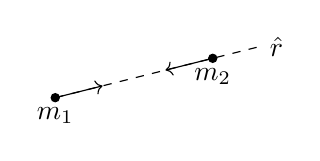
\begin{tikzpicture}\fill(0,0)circle(.06)node[below]{$m_1$};\fill(2,.5)circle(.06)node[below]{$m_2$};\draw[dashed](0,0)--(2.6,.65)node[right]{$\hat r$};\draw[->](0,0)--(.6,.15);\draw[->](2,.5)--(1.4,.35);\end{tikzpicture}\end{center}
\subsection*{Leggi di Keplero}
\begin{enumerate}\item Le orbite dei pianeti sono piane e formano un'ellisse con il Sole che occupa uno dei 2 fuochi.
\item Il raggio vettore descrive aree proporzionali ai tempi impiegati a descriverle.
\item $T^2\propto a^3$ ($T^2=\dfrac{4\pi^2}{GM}r^3$, $GM$ cost.).\end{enumerate}
\[E_K=-\tfrac12G\frac{Mm}{r}<0\quad\text{(cerchio)}.\]
\[E_m=-\frac{(Mm)^{[?]}G^2}{M+m}\,\frac{1}{2J^2}(1-e^2).\]
$E>0\Rightarrow$ il corpo non ritorna; $E<0\Rightarrow$ il corpo ritorna su orbita.
\nota{La fonte scrive un'energia con pedice $K$ negativa e una formula successiva con simboli poco nitidi: $J$, il pedice $m$ e l'esponente sul prodotto $Mm$ sono letture incerte (esponente segnalato con $[?]$). Le espressioni sono mantenute senza correggerle.}
% Pagina originale 8
\orig{8}\section*{Pendolo fisico}
\[\tau=-Mgl\sin\theta,\qquad \theta(t)=\theta_{\max}\cos(\omega t+\varphi),\qquad \omega=\sqrt{\frac{Mgl}{I}}.\]
\[T=\frac{2\pi}{\omega}=2\pi\sqrt{\frac{I}{Mgl}}.\]
\section*{Fisica 2}\subsection*{Legge di Coulomb}
\[\vv F=k\frac{q_1q_2}{r^2}\hat r\quad\text{con }k=\frac1{4\pi\varepsilon_0}\quad[\mathrm N].\]
\[\varepsilon_0=8.85\cdot10^{-12}\quad(\varepsilon_0\leftarrow\text{nel vuoto}),\qquad \varepsilon_r>1\quad(\varepsilon_0\varepsilon_r\leftarrow\text{in un materiale}).\]
\subsection*{Campo elettrostatico}
\[E=\frac q{4\pi\varepsilon_0r^2},\qquad
\lambda=\frac{\dd q}{\dd x}=\frac{q_{\mathrm{tot}}}{L},\quad
\sigma=\frac{\dd q}{\dd S}=\frac{q_{\mathrm{tot}}}{A},\quad
\rho=\frac{\dd q}{\dd V}=\frac{q_{\mathrm{tot}}}{V}.\]
Barra: lunghezza $L$; rettangolo: $A=ab$; parallelepipedo: $V=abc$.
\begin{center}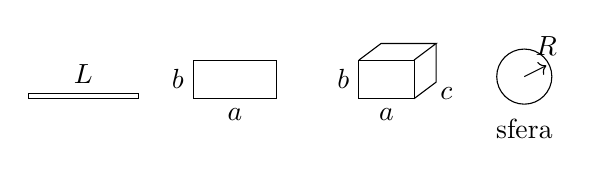
\begin{tikzpicture}[scale=.7]
\draw(0,0)rectangle(2,.1);\node[above]at(1,.1){$L$};
\draw(3,0)rectangle(4.5,.7);\node[below]at(3.75,0){$a$};\node[left]at(3,.35){$b$};
\draw(6,0)rectangle(7,.7);\draw(6,.7)--(6.4,1)--(7.4,1)--(7,.7);\draw(7.4,1)--(7.4,.3)--(7,0);\node[below]at(6.5,0){$a$};\node[left]at(6,.35){$b$};\node[right]at(7.3,.1){$c$};
\draw(9,.4)circle(.5);\draw[->](9,.4)--(9.4,.6)node[above]{$R$};\node[below]at(9,-.2){sfera};
\end{tikzpicture}\end{center}

\begin{center}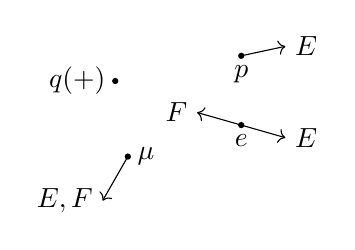
\begin{tikzpicture}[scale=.8]\fill(0,0)circle(.05)node[left]{$q(+)$};\fill(2,.4)circle(.05)node[below]{$p$};\draw[->](2,.4)--(2.7,.55)node[right]{$E$};\fill(2,-.7)circle(.05)node[below]{$e$};\draw[->](2,-.7)--(2.7,-.9)node[right]{$E$};\draw[->](2,-.7)--(1.3,-.5)node[left]{$F$};\fill(.2,-1.2)circle(.05)node[right]{$\mu$};\draw[->](.2,-1.2)--(-.2,-1.9)node[left]{$E,F$};\end{tikzpicture}\end{center}
\[\dd E=\frac{\dd q}{4\pi\varepsilon_0r^2}\Rightarrow E=\int\frac{\dd q}{4\pi\varepsilon_0r^2}.\]
\subsection*{Legge di Gauss}
\[\Phi_E=\frac{Q_{\mathrm{int}}}{\varepsilon_0},\qquad \Phi_E=\int E\,\dd S.\]
Sfera cava:
\[E(r)=\begin{cases}\dfrac q{4\pi\varepsilon_0r^2}&r\ge R,\\0&r<R.\end{cases}\]
Sfera piena isolante:
\[E(r)=\begin{cases}\dfrac{|\rho|r}{3\varepsilon_0}&r\le R,\\[4pt]\dfrac{|q|}{4\pi\varepsilon_0r^2}=\dfrac{|\rho|R^3}{3\varepsilon_0r^2}&r>R.\end{cases}\]
\nota{Una prima formula per l'interno della sfera cava è cancellata e sostituita da $0$.}
% Pagina originale 9
\orig{9}
Nei materiali conduttori le cariche si distribuiscono sulla superficie.
\[|E(P)|=\begin{cases}0&P\in\Sigma\quad\text{(spazio interno della figura, sfera)},\\>0&\text{altrimenti}.\end{cases}\]
\textbf{Disco}, raggio $R$, punto sull'asse a distanza $z$:
\[E(z)=\frac q{2\pi\varepsilon_0R^2}\left(1-\frac z{\sqrt{z^2+R^2}}\right).\]
\textbf{Anello}, punto sull'asse a distanza $x$:
\[E(x)=\frac q{4\pi\varepsilon_0}\frac{x}{(a^2+x^2)^{3/2}}.\]
\begin{center}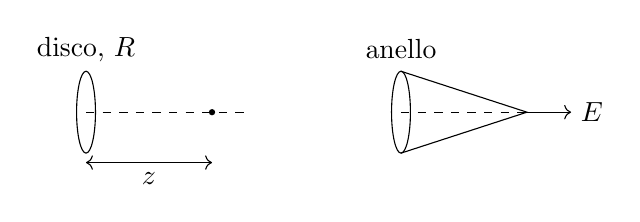
\begin{tikzpicture}[scale=.8]\draw(0,0)ellipse(.15 and .65);\draw[dashed](0,0)--(2.5,0);\fill(2,0)circle(.05);\draw[<->](0,-.8)--node[below]{$z$}(2,-.8);\node at (0,1){disco, $R$};\begin{scope}[xshift=5cm]\draw(0,0)ellipse(.15 and .65);\draw(0,.65)--(2,0)--(0,-.65);\draw[dashed](0,0)--(2.5,0);\draw[->](2,0)--(2.7,0)node[right]{$E$};\node at (0,1){anello};\end{scope}\end{tikzpicture}\end{center}
\textbf{Piano:}\quad $E(x)=\dfrac\sigma{2\varepsilon_0}$.
\begin{center}\begin{tikzpicture}[scale=.7]\draw(0,-.7)--(0,.7);\draw[<->](-1,0)--(-.2,0);\draw[<->](.2,0)--(1,0);\node at (0,-1){piano};\begin{scope}[xshift=4cm]\draw(0,-.7)--(0,.7);\draw(1.5,-.7)--(1.5,.7);\node[below]at(0,-.7){$0$};\node[below]at(1.5,-.7){$a$};\draw[->](.3,0)--(1.2,0);\draw[<->](-1,0)--(-.2,0);\draw[<->](1.7,0)--(2.5,0);\end{scope}\end{tikzpicture}\end{center}
Due piani:
\[E(x)=\begin{cases}0&x\notin(0,a),\\\dfrac\sigma{\varepsilon_0}&x\in(0,a).\end{cases}\]
\begin{center}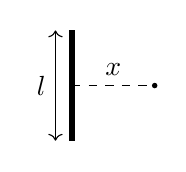
\begin{tikzpicture}[scale=.7]\draw[line width=2pt](0,-1)--(0,1);\draw[<->](-.3,-1)--node[left]{$l$}(-.3,1);\fill(1.5,0)circle(.05);\draw[dashed](0,0)--(1.5,0)node[midway,above]{$x$};\end{tikzpicture}\end{center}
Filo finito, lunghezza indicata $l$ e distanza $x$:
\[E(x)=\frac{\lambda l}{4\pi\varepsilon_0x\sqrt{x^2+l^2}}\quad\text{[formula marginale parzialmente tagliata]},\qquad
\left(E(x)=\frac\lambda{2\pi\varepsilon_0x}\right).\]
\nota{La formula sul margine destro è tagliata dal bordo della pagina: il numeratore sembra $\lambda l$ e il denominatore $4\pi\varepsilon_0x\sqrt{x^2+l^2}$; i fattori non leggibili non sono ricostruiti.}
\textbf{Forza elettrica:}\quad $F=qE$.
\[\dd W=F\,\dd s\Rightarrow W=L=\int F\,\dd s.\]
\subsection*{Energia potenziale elettrica}
\[U_{\mathrm{el}}=qV,\qquad L=-\Delta U.\]
\subsection*{Potenziale elettrico}
\[V=Ed,\qquad V=\int_r^{\infty}E\,\dd s,\qquad V(r)=\frac q{4\pi\varepsilon_0r}.\]
Rispetto ad un punto distante $r$.
% Pagina originale 10
\orig{10}\section*{Circuiti}
\subsection*{Capacità}
\[C=\frac q{\Delta V},\qquad\Delta V=\frac qC,\qquad q=C\Delta V.\]
\[\frac1{C_{\mathrm{eq}}}=\sum_i\frac1{C_i}\quad\text{in serie};\qquad
C_{\mathrm{eq}}=\sum_i C_i\quad\text{in parallelo}.\]
\begin{center}\begin{circuitikz}[scale=.7]\draw(0,0)to[C,l=$C_1$](2,0)to[C,l=$C_2$](4,0);\draw(5,0)to[C,l=$C_{\rm eq}$](7,0);\node at(4.5,0){$\Leftrightarrow$};\draw(0,-2)--(0,-1.4)to[C](4,-1.4)--(4,-2);\draw(0,-2)--(0,-2.6)to[C](4,-2.6)--(4,-2);\draw(5,-2)to[C,l=$C_{\rm eq}$](7,-2);\node at(4.5,-2){$\Leftrightarrow$};\end{circuitikz}\end{center}
\[U=\tfrac12C\Delta V^2,\qquad C=\varepsilon_0\frac Ad.\]
Condensatore piano: armature di area $A$, distanti $d$.
\begin{center}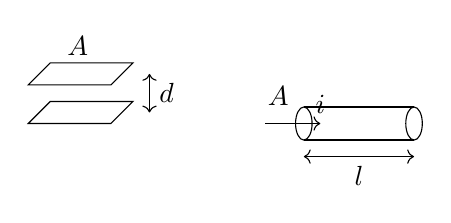
\begin{tikzpicture}[scale=.7]
\draw(0,0)--(1.5,0)--(1.9,.4)--(.4,.4)--cycle;\draw(0,.7)--(1.5,.7)--(1.9,1.1)--(.4,1.1)--cycle;\draw[<->](2.2,.2)--node[right]{$d$}(2.2,.9);\node at(.9,1.4){$A$};
\begin{scope}[xshift=5cm]\draw(0,0)ellipse(.15 and .3);\draw(2,0)ellipse(.15 and .3);\draw(0,.3)--(2,.3);\draw(0,-.3)--(2,-.3);\draw[->](-.7,0)--(.3,0)node[above]{$i$};\node[left]at(-.1,.5){$A$};\draw[<->](0,-.6)--node[below]{$l$}(2,-.6);\end{scope}
\end{tikzpicture}\end{center}

\subsection*{Resistenza}
\[R=\rho\frac lA.\]
\textbf{Legge di Ohm:}\quad $V=Ri$, $R=V/i$, $i=V/R$.
\[R_{\mathrm{eq}}=\sum_iR_i\quad\text{in serie};\qquad
\frac1{R_{\mathrm{eq}}}=\sum_i\frac1{R_i}\quad\text{in parallelo}.\]
\begin{center}\begin{circuitikz}[scale=.7]\draw(0,0)to[R](2,0)to[R](4,0);\draw(5,0)to[R,l=$R_{\rm eq}$](7,0);\node at(4.5,0){$\Leftrightarrow$};\draw(0,-2)--(0,-1.4)to[R](4,-1.4)--(4,-2);\draw(0,-2)--(0,-2.6)to[R](4,-2.6)--(4,-2);\draw(5,-2)to[R,l=$R_{\rm eq}$](7,-2);\node at(4.5,-2){$\Leftrightarrow$};\end{circuitikz}\end{center}
\subsection*{Corrente}
\[i=\frac{\dd q}{\dd t}\quad\left(=\frac qt\text{ in cond. stazionarie}\right),\qquad J=\frac iA.\]
Sezione del filo $A$, corrente $i$.
\subsection*{Potenza}
\[P=Ri^2=\frac{V^2}{R}=Vi.\]
\textbf{Kirchhoff:}\quad $\sum i=0$ $\forall$ nodo; $\sum V=0$ $\forall$ maglia.
\begin{center}\begin{circuitikz}[scale=.65]\draw(0,0)to[battery1](0,2)to[R](2,2)to[R](4,2)to[battery1](4,0)--(0,0);\draw(2,2)to[R](2,0);\fill(2,2)circle(.06);\draw[->](2,2)--(1,-.7);\end{circuitikz}\quad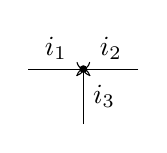
\begin{tikzpicture}[scale=.7]\fill(0,0)circle(.07);\draw[->](-1,0)--(0,0)node[midway,above]{$i_1$};\draw[->](1,0)--(0,0)node[midway,above]{$i_2$};\draw[->](0,-1)--(0,0)node[midway,right]{$i_3$};\end{tikzpicture}\end{center}
Prima ipotesi di correnti entranti $\Rightarrow$ eq. delle maglie + eq. correnti $\Rightarrow i_1>0$, $i_2>0$, $i_3<0$ (verso sbagliato).

Nodo aggiornato: $i_1$, $i_2$ entranti, $i_3$ uscente. Caduta di tensione: $\Delta V$ nel verso della corrente lungo la resistenza (orizzontale verso destra; verticale verso l'alto nel disegno).
% Pagina originale 11
\orig{11}\section*{Magnetismo}
\[B=\frac{\mu_0i}{2\pi h}\quad\text{filo infinito},\qquad \mu_0=4\pi\cdot10^{-7}.\]
\begin{center}\begin{tikzpicture}\draw[->](0,-.5)--(0,1)node[above]{$i$};\draw(1,0)rectangle(1.3,.5);\draw[<->](0,-.3)--node[below]{$h$}(1,-.3);\end{tikzpicture}\end{center}
\textbf{Legge di Biot--Savart:}\quad
$\dd\vv B=\dfrac{\mu_0i\,\dd\vv s\cdot\hat r}{4\pi r^2}$.
\nota{Il segno fra $\dd\vv s$ e $\hat r$ nella fonte sembra un punto: si mantiene $\cdot$, pur essendo la formula vettoriale usuale diversa.}
\textbf{Effetto Hall:}\quad $j=\dfrac iA=ne v_d$.
\[v_d=\text{velocità di deriva}=\frac j{ne}=\frac i{neA}.\]
\[E=vB.\]
\nota{Accanto a $E=vB$ c'è uno schizzo cancellato e non leggibile, non ricostruito.}
\[\vv B=\varepsilon_0\mu_0\vv v\wedge\vv E=\frac1{c^2}\vv v\wedge\vv E.\]
\begin{center}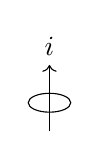
\begin{tikzpicture}[scale=.6]\draw(0,0)ellipse(.45 and .2);\draw[->](0,-.6)--(0,.8)node[above]{$i$};\end{tikzpicture}\end{center}
\textbf{Legge di Ampere:}\quad $\displaystyle\oint B\,\dd s=\mu_0i$.

\textbf{Legge di Faraday:}\quad $\displaystyle\varepsilon=-\frac{\dd\Phi_B}{\dd t}$;
$\displaystyle\Phi_B=\int_S B\,\dd s$, $(\varepsilon=-BLv)$.
\subsection*{Forza di Lorentz}
\[\vv F_q=q\vv v\wedge\vv B,\qquad \vv F_l=i\vv l\wedge\vv B.\]
\[q\frac{\dd\vv x}{\dd t}\wedge\vv B=\frac{\dd q}{\dd t}\vv x\wedge\vv B=i\vv x\wedge\vv B.\]
\begin{center}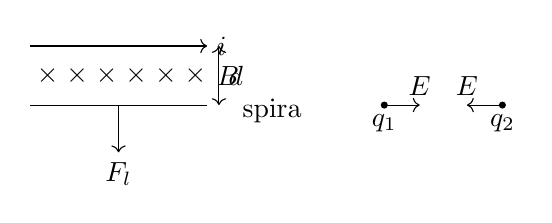
\begin{tikzpicture}[scale=.75]\draw[->](0,1)--(3,1)node[right]{$i$};\draw(0,0)--(3,0);\draw[<->](3.2,0)--node[right]{$d$}(3.2,1);\foreach\x in {.3,.8,1.3,1.8,2.3,2.8}\node at(\x,.5){$\times$};\node[right]at(3,.5){$B$};\draw[->](1.5,0)--(1.5,-.8)node[below]{$F_l$};\node at(4.1,-.1){spira};\begin{scope}[xshift=6cm]\fill(0,0)circle(.06)node[below]{$q_1$};\fill(2,0)circle(.06)node[below]{$q_2$};\draw[->](0,0)--(.6,0)node[above]{$E$};\draw[->](2,0)--(1.4,0)node[above]{$E$};\end{scope}\end{tikzpicture}\end{center}
Dove c'è la carica c'è un campo elettrico.

Dove c'è corrente c'è un campo elettrico.
\nota{L'ultima frase scrive ``elettrico'', mantenuto come nella fonte.}
% Pagina originale 12
\orig{12}
\begin{center}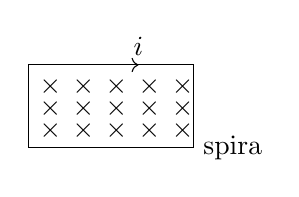
\begin{tikzpicture}[scale=.7]\draw(0,0)rectangle(3,1.5);\draw[->](1,1.5)--(2,1.5)node[above]{$i$};\foreach\x in {.4,1,1.6,2.2,2.8}\foreach\y in {.3,.7,1.1}\node at(\x,\y){$\times$};\node[right]at(3,0){spira};\end{tikzpicture}\end{center}
\[\frac{\dd\Phi_B}{\dd t}\ne0\Rightarrow i\text{ indotta (con verso opposto)}\Rightarrow\varepsilon\ne0.\]
\begin{center}\begin{tabular}{lll}
&Campo $B$&Corrente $i$\\
Prima coppia di schizzi&entrante&orario\\
&uscente&antiorario\\
Seconda coppia di schizzi&entrante&antiorario\\
&uscente&orario
\end{tabular}\end{center}
\begin{center}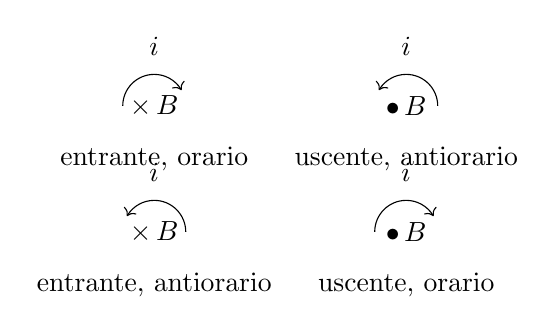
\begin{tikzpicture}[scale=.8]
\node at(0,0){$\times\,B$};\draw[->](-.5,0)arc(180:30:.5);\node[above]at(0,.65){$i$};\node[below]at(0,-.5){entrante, orario};
\begin{scope}[xshift=4cm]\node at(0,0){$\bullet\,B$};\draw[->](.5,0)arc(0:150:.5);\node[above]at(0,.65){$i$};\node[below]at(0,-.5){uscente, antiorario};\end{scope}
\begin{scope}[yshift=-2cm]\node at(0,0){$\times\,B$};\draw[->](.5,0)arc(0:150:.5);\node[above]at(0,.65){$i$};\node[below]at(0,-.5){entrante, antiorario};\end{scope}
\begin{scope}[xshift=4cm,yshift=-2cm]\node at(0,0){$\bullet\,B$};\draw[->](-.5,0)arc(180:30:.5);\node[above]at(0,.65){$i$};\node[below]at(0,-.5){uscente, orario};\end{scope}
\end{tikzpicture}\end{center}
\nota{Le due coppie di frecce circolari della fonte riportano versi opposti, senza una condizione testuale che le distingua; entrambe sono conservate.}
Se $B$ costante nel tempo ($\Phi_B$ cost.) allora
\[\frac{\dd\Phi_B}{\dd t}=0\Rightarrow\varepsilon=0\quad\text{nessuna f.e.m.}\]
Forza elettromotrice. Un generatore è un esempio di f.e.m.
\begin{center}\begin{circuitikz}[scale=.6]\draw(0,0)to[battery1,l=$\varepsilon$](0,2)--(3,2)to[R](3,0)--(0,0);\draw(5,1)to[C](7,1)to[R](9,1);\end{circuitikz}\end{center}
\[i(t)=i_0e^{-t/RC}\quad\text{carica/scarica cond.}\]
Due condensatori collegati:
\[\begin{cases}q_1'+q_2'=q_1-q_2&\text{cons. della carica},\\[4pt]
\dfrac{q_1'}{C_1}=\dfrac{q_2'}{C_2}&\text{cond. d'equilibrio}.\end{cases}\]
\begin{center}\begin{circuitikz}[scale=.6]\draw(0,0)to[C,l=$C_1$](0,2)--(3,2)to[C,l=$C_2$](3,0)--(0,0);\node[left]at(0,.4){$+$};\node[left]at(0,1.6){$-$};\node[right]at(3,.4){$+$};\node[right]at(3,1.6){$-$};\end{circuitikz}\end{center}
\subsection*{Induttanza}
\begin{center}\begin{circuitikz}\draw(0,0)to[L](3,0);\end{circuitikz}\end{center}
\[L=\frac{N\Phi_B}{i},\qquad B=\mu_0ni\quad\text{nel solenoide}.\]
\[\varepsilon=-\underbrace L_{\text{coeff. di autoinduzione}}\frac{\dd i}{\dd t}.\]
% Pagina originale 13
\orig{13}\section*{Eq. di Maxwell}
\[\begin{aligned}
\nabla\cdot\vv E&=\frac\rho{\varepsilon_0},&\nabla\times\vv E&=-\frac{\partial\vv B}{\partial t},\\
\nabla\cdot\vv B&=0,&\nabla\times\vv B&=\mu_0\vv j+\mu_0\varepsilon_0\frac{\partial\vv A}{\partial t}.
\end{aligned}\]
\nota{Nell'ultima derivata la lettera manoscritta sembra $A$ (con freccia), anziché $E$; è mantenuta e segnalata, senza correzione tacita.}
\section*{Carica e scarica}
\subsection*{Carica}
\[q(t)=\underbrace{C\varepsilon}_{q_0}(1-e^{-t/RC}),\qquad
i(t)=\underbrace{\frac\varepsilon R}_{i_0}e^{-t/RC},\qquad
V_C(t)=\varepsilon(1-e^{-t/RC}).\]
\begin{center}\begin{tikzpicture}[scale=.8]\draw[->](0,0)--(4,0)node[right]{$t$};\draw[->](0,0)--(0,2);\draw[dashed](0,1.5)--(4,1.5);\draw[domain=0:4,samples=50]plot(\x,{1.5*(1-exp(-\x))});\node[right]at(4,1.3){$V$};\begin{scope}[yshift=-3cm]\draw[->](0,0)--(4,0)node[right]{$t$};\draw[->](0,0)--(0,2);\draw[domain=0:4,samples=50]plot(\x,{1.5*exp(-\x)});\node[right]at(4,.2){$i$};\end{scope}\end{tikzpicture}\end{center}
\subsection*{Scarica}
\[q(t)=q_0e^{-t/RC},\qquad
V_C(t)=V_0e^{-t/RC}=\frac{q_0}{C}e^{-t/RC},\qquad
i(t)=\frac{V_0}{R}e^{-t/RC}.\]
\end{document}
